\documentclass[12pt]{article}

\usepackage[T1]{fontenc}
\usepackage{amsfonts, amsmath, amssymb}
\usepackage{multirow}
\usepackage{epsfig}
\usepackage{subfigure}
\usepackage{subfloat}
\usepackage{graphicx}
\usepackage{hyperref}
\usepackage{parskip}
\usepackage{booktabs}
\usepackage{longtable}
\usepackage[utf8]{inputenc}
\usepackage[english]{babel}
% \usepackage[document]{ragged2e}
\usepackage{verbatim, rotating, paralist}
\usepackage{enumerate}
\usepackage{float}

\usepackage{natbib}


\usepackage{pdfsync}
\usepackage{latexsym}
\usepackage{amsthm}
\usepackage{mathabx}

\usepackage{stmaryrd}
\usepackage{mathrsfs}
\usepackage{dsfont}
\usepackage{fancyhdr}
\usepackage{color}

\usepackage{parskip}
\usepackage{anysize, indentfirst, setspace}
\usepackage[right=1.75cm, left=1.75cm, top=3cm, bottom=3cm]{geometry}
\usepackage{appendix}

\usepackage{enumitem}
\setlist{nosep}
\author{White Team \\ Chenxi Rong, Xiaoquan Liu, Zhanyi Lin, Fabian Schmid}

\renewcommand{\topfraction}{.85}
\renewcommand{\bottomfraction}{.7}
\renewcommand{\textfraction}{.15}
\renewcommand{\floatpagefraction}{.66}
\renewcommand{\dbltopfraction}{.66}
\renewcommand{\dblfloatpagefraction}{.66}




% \pagestyle{fancyplain}
% \rhead{\hfill \small \emph{MIDS NUMBER -- Fall 2019}}
\cfoot{}

% \renewcommand{\headrulewidth}{0pt}


\title{Opioid project strategy outline}

%-------------------------- BEGIN DOCUMENT ----------------------------------%
\begin{document}
\maketitle

\section{Topic}

%\emph{What problem are you (or your stakeholder) trying to addres?}

We want to address the problem that a high number of  opioids are prescribed in the United States. This development induces severe consequences like more overdose deaths and opioid addicts over the last twenty years.
\vspace*{0.5cm}

\section{Project Question}
%emph{What specific question are you seeking to answer with this project?}
In this project we want to answer the following two specific questions: 
\begin{itemize}
\item What is the effect of opioid drug prescription regulations on the volume of opioids prescribed?

\item What is the effect of opioid drug prescription regulations on drug overdose deaths?

\end{itemize}

For that, we will analyze three policies implemented on the state level in Washington, Texas, and Florida which came into effect between 2007 and 2012. 

\vspace*{0.5cm}
\section{Project Hypothesis}
%\emph{What is your hypothesized answer to your question?}

We hypothesize that the answers to the two project questions are:
\begin{itemize}
\item Opioid drug prescription regulations decrease the volume of opioids prescribed.

\item Opioid drug prescriptions regulations increase drug overdose deaths in the short to medium run as opioid addicts substitute prescription opioids with more dangerous non-prescription opioids.
\end{itemize}

\vspace*{0.5cm}




\section{Model Results}
%\emph{One of the hardest parts of developing a good data science project is developing a question that is actually answerable. Perhaps the best way to figure out if your question is answerable is to see if you can imagine what an answer to your question would look like. Below, draw the graph, regression table, etc. that you would consider to be an answer to your question. Then draw it again, so you have a model result for if your hypothesized answer is true, and a model result for if your hypothesized answer is false. (If the answer to your question is continuous, not discrete (like: what is the level of inequality in the United States), draw it for high values (high inequality) and low values (low inequality)).}

In the final report, the graphics below will be presented separately for two different policy interventions in Florida and Washington. In addition, similar graphics will be generated using drug overdose mortality per capita on the y-axis. For that, three policies in Florida, Washington, and Texas will be analyzed. All graphics will include standard error bands.


\begin{minipage}{0.5\textwidth}
\centering
\textbf{Result if the hypothesis is true}
\end{minipage}
\begin{minipage}{0.5\textwidth}
\centering
\textbf{Result if the hypothesis is false}
\end{minipage}

\begin{figure}[H]
    \centering
    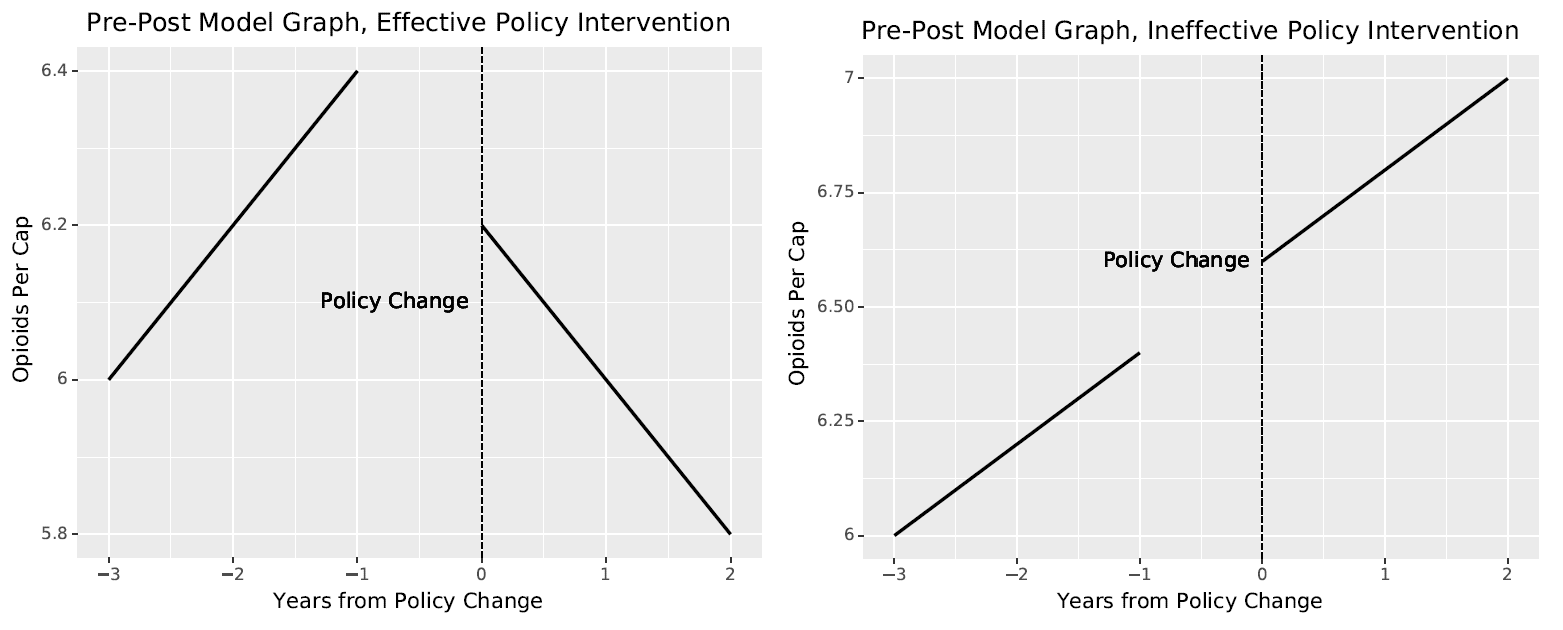
\includegraphics[scale=.5]{41_project_strategy_potential_model_results_prepost.png}
    \caption{Potential model results pre-post comparison }
    \label{fig:prepost}
\end{figure}

\begin{figure}[h]
    \centering
    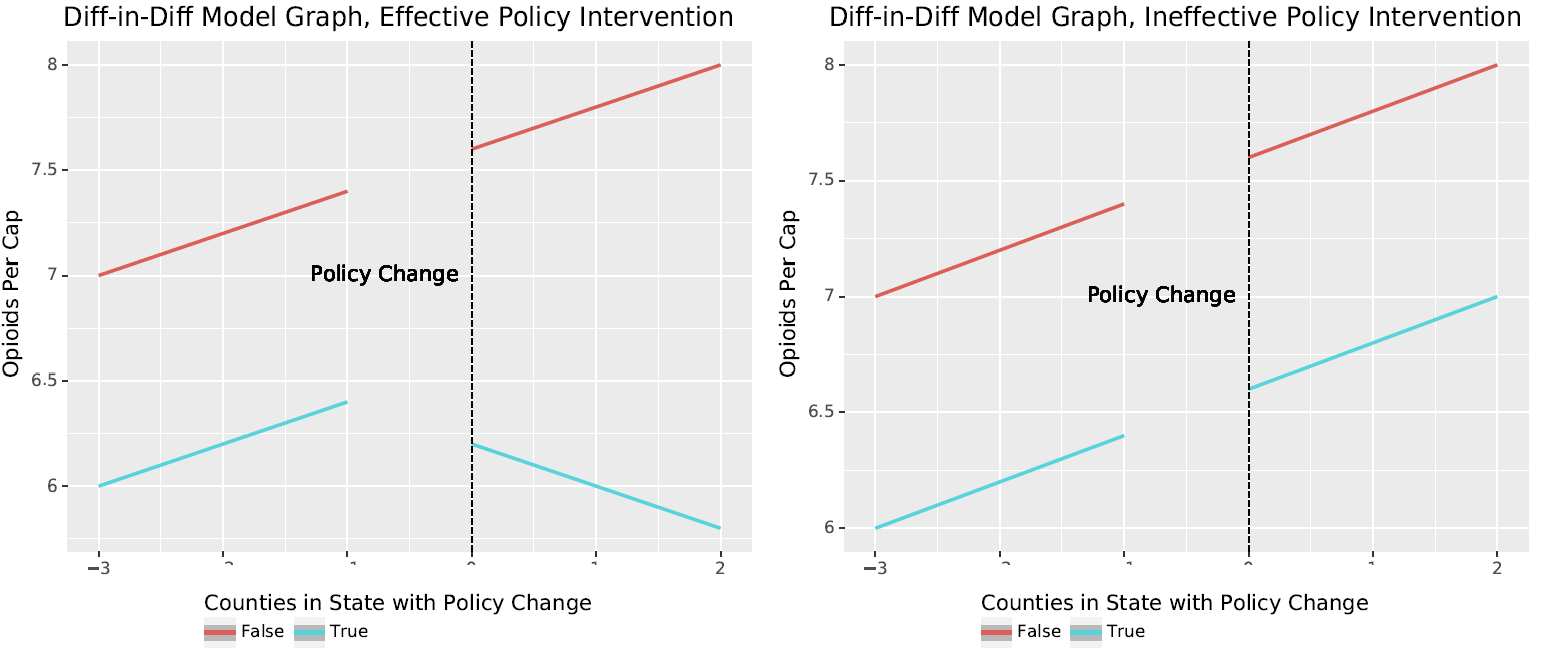
\includegraphics[scale=.5]{41_project_strategy_potential_model_results_did.png}
    \caption{Potential model results difference-in-difference comparison }
    \label{fig:did}
\end{figure}



\vspace*{1cm}
\section{Final Variables Required}

%\emph{Now that you've specified what an answer to your question looks like, what data do you need to generate that answer.}

%\emph{For each variable, define both the variable you need \textbf{and} the population for which you need the variables to be defined.}

%\emph{You don't have to be too specific (``I need variable 7 from the NHGIS 2019 census 1\% sample release'') -- just define it in the most general terms that are still specific enough to meet your needs (e.g. I need income data for a nationally representative sample of US citizens). }
%\pagebreak

A single row in the final data set will contain one observation for one county for one year. All data should be available before and after the policy intervention to conduct the pre-post comparison (Florida February 2010, Texas January 2007, Washington January 2012). For the difference-in-difference approach data is required for both, US counties which are affected by the policy intervention and for those which are unaffected.  The following variables are required in the final data set to conduct the analysis:

\begin{itemize}

\item Opioid drug prescriptions per capita per county per year
	\begin{itemize}
	\item Absolute opioid drug prescriptions per county per year
	\item County population size per year
	\end{itemize}
\item Drug overdose mortality numbers per capita per county per year
	\begin{itemize}
	\item Absolute drug overdose mortality numbers per county per year
	\item County population size per year
	\end{itemize}
\item Binary variable which indicates whether the observation is in a state with a policy change (for difference-in-difference)

\item County FIPS code

\item Year



\end{itemize}

\section{Data Sources}

%\emph{Finally, given the variables you need for your analysis, what actual data sources do you think will have the data you need?}

%\emph{In specifying the datasets you need, if you list more than one \textbf{also} indicate how you think you can relate these datasets (i.e. if you're gonna merge them, what variables do you think those datasets will provide that will allow you merge them? There's no use saying ``I'll merge this political survey with medical records of who has received bad care'' if the political survey doesn't provide identifying information you can use to link survey respondents to medical records, even if you have both the survey and medical records!)}

The above described required variables can be obtained by using the following data sources:

\begin{itemize}
	\item Drug overdose death data by the US Vital Statistics records
	\item Prescription opioid drug shipments by the Washington Post
	\item FIPS codes based on a file by the \href{https://www2.census.gov/geo/docs/reference/codes/files/national_county.txt}{US census}
	\item \href{https://www.census.gov/programs-surveys/popest/data.html}{US census} population data
\end{itemize}

All these data sets need at least a location name (to infer the county) and a temporal unit (to infer the year). The data sets will be merged based on the county FIPS codes and the year. FIPS codes are already included in the population data set and the US Vital Statistics records. Based on the county and state name, FIPS codes will be merged with the prescription opioid drug shipment data. Besides that, the raw data must be aggregated on the county-year level so that the data is available for our preferred unit of observation.
\vspace*{1cm}


\section{Task Assignment}

\begin{center}
\begin{tabular}{ l | l l}
\textbf{Step}  & \textbf{Writes initial code} & \textbf{Reviews code}\\ \hline
 Import data & Fabian & Zhanyi\\  
 Clean and aggregate data & Fabian & Zhanyi\\
 Merge data & Zhanyi \& Chenxi & Fabian \\
 Analyze data & Zhanyi \& Chenxi & Xiaoquan \\
 Create graphs & Chenxi \&  Xiaoquan & Xiaoquan\\
 Report(e.g. motivation, conclusion) & Xiaoquan & Chenxi \\
\end{tabular}
\end{center}

\end{document}
